\section{Set up analysis}
\label{setupanalysis}
Once Romeo is properly installed on the computer, you can start to fill it with your data, in order to perform an analysis. Before this, you need to import your images and eventually their relative mask, create your group of Subjects\g{}, your Protocols\g{} and your Datasets\g{}. Please read this section to get more information about these operations.\\
This chapter contains the following sections:
\begin{itemize}
\item \textbf{About Subjects}
\item \textbf{About groups of Subjects}
\item \textbf{About Protocols}
\item \textbf{About Datasets}
\end{itemize}

\subsection{About Subjects}
\label{aboutsubject}
This section contains the procedures to create and manage the Subjects\g{}.

\subsubsection{Create Subject}
\label{createsubject}
The creation of a new Subject\g{} is assigned to the Subjects\g{} creation window.\\
From the main window of Romeo, select the \textit{New Subject} button or choose the right one in the toolbar (see \ref{environment}). The Subjects\g{} creation window (fig. \ref{createsubjectimg}), is composed of one panel containing a form in which the user have to insert the information about the \subject{}. In any moment, the user can go back to the main window by selecting the \textit{Back} button.
\begin{figure}[!h]
\begin{center}
\includegraphics[scale=0.4]{./Images/NewSubjectView}
\caption{\textit{Subject creation window}}
\label{createsubjectimg}
\end{center}
\end{figure}
\\To create a new Subject\g{}, follow these instructions:
\begin{itemize}
\item From the Subjects\g{} creation window, type a unique name in the \textit{Subject Name} field. That name will be the name of the \subject{};
\item Select the image type that will be imported in the Subject\g{}. The type could be: 2D, 3D, 2D-t, 3D-t;
\item Select the image to import by selecting the \textit{Search} button next to the \textit{Add File} field and navigating the file system;
\item Import a mask\g{} selecting it by clicking the \textit{Search} button next to the \textit{Add Mask} field and navigating the file system, if necessary;
\item Confirm the operation by clicking the \textit{Save} button. Romeo will report an error message if not all the required fields are fulfilled or the name chosen for the Subject\g{} is already present in Romeo.
\end{itemize}

\subsubsection{Visualize Subjects}
\label{visulizesubjects}
The visualization of the details of a \subject{} is assigned to the Subject\g{} visualization window.\\
From the main window of Romeo, select the \textit{View Subjects} button or choose the right one in the toolbar (see \ref{environment}). The Subject\g{} visualization window (fig. \ref{visualizesubjectimg}), is composed of two panels. The left one contains the list of Subjects\g{} stored in Romeo, ordered by creation data (by default, from the oldest one, to the newest). For each Subject\g{} it is specified:
\begin{itemize}
\item \textbf{Name:} the name of the Subject\g{};
\item \textbf{Type:} the type of the Subject\g{} (2D, 3D, 2D-t, 3D-t);
\item \textbf{Mask:} display \textit{yes} if a mask was associated to the image, \textit{no} otherwise;
\item \textbf{Creation date:} the date and time in which the Subject\g{} was created.
\end{itemize}
The right panel contains the details of the selected Subject\g{}. It shows a preview of the image associated to the \subject{} and the list of groups that include such \subject{}. In any moment, the user can go back to the main window by selecting the \textit{Back} button.
\begin{figure}[!h]
\begin{center}
\includegraphics[scale=0.4]{./Images/ViewSubjects}
\caption{\textit{Subject visualization window}}
\label{visualizesubjectimg}
\end{center}
\end{figure}
\pagebreak
\\To visualize the Subjects\g{} present into Romeo, follow these instructions:
\begin{itemize}
\item From the Subject\g{} visualization window, select the Subject\g{} of interest, from the list present in the left panel of the window;
\item The \textbf{Details} panel will show a preview of the image and a list of groups in which this Subject\g{} is present.
\end{itemize}

\subsection{About groups of Subjects}
\label{aboutgroups}
This section contains the procedures to create and manage the groups of Subjects\g{}.

\subsubsection{Create a group of Subjects}
\label{creategroup}
The creation of a new group of Subjects\g{} is assigned to the group of Subjects\g{} creation window.\\
From the main window of Romeo, select the \textit{New Group} button or choose the right one in the toolbar (see \ref{environment}). The group of Subjects\g{} creation window (fig. \ref{creategroupimg}) is composed of two panels.\\
The left one contains the information about the group that is going to be created (Name and Type). The right panel contains the list of Subjects\g{} actually stored in Romeo (filtered according to the selected type), plus the utility buttons \textit{Select All} and \textit{Deselect All}. In any moment, the user can go back to the main window by selecting the \textit{Back} button.
\begin{figure}[!h]
\begin{center}
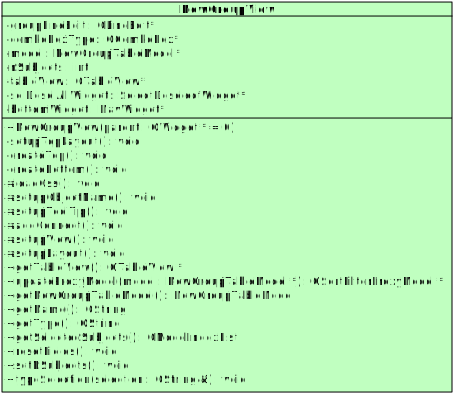
\includegraphics[scale=0.4]{./Images/NewGroupView}
\caption{\textit{Group of Subjects creation window}}
\label{creategroupimg}
\end{center}
\end{figure}
\pagebreak
\\To create a new group of Subjects\g{}, follow these instructions:
\begin{itemize}
\item From the group of Subjects\g{} creation window, type a unique name in the \textit{Group name} field. That name will be the name of the group;
\item Select the type of the Subjects\g{} that will be included in the group from the \textit{Type} drop-down menu. A list of Subjects\g{} with that type, will be listed in the right panel;
\item Select the Subjects\g{} that have to be included into the group, from the list of Subjects\g{};
\item Confirm the operation by selecting the \textit{Save} button. Romeo will report an error message if the name chosen for the group is already present in Romeo or not all the required fields are fulfilled.
\end{itemize}

\subsubsection{Manage groups of Subjects}
\label{managegroups}
Romeo allows the user to visualize the details of the stored groups of Subjects\g{} and permits their removal or modification. These features are assigned to the groups of Subjects\g{} managing window.\\
From the main window of Romeo, select the \textit{Manage Groups} button or choose the right one in the toolbar (see \ref{environment}). The groups of Subjects\g{} managing window (fig. \ref{managegroupimg}), is composed of two panels. The left one contains the list of the groups of Subjects\g{} stored in Romeo, ordered by creation data (by default, from the oldest one, to the newest). For each group it is specified:
\begin{itemize}
\item \textbf{Name:} the name of the group;
\item \textbf{Type:} the type of the Subjects\g{} associated with it (2D, 3D, 2D-t, 3D-t);
\item \textbf{Subjects:} the number of Subjects\g{} associated with it;
\item \textbf{Creation Date:} the date and time in which the group of Subjects\g{} was created.
\end{itemize}
The right panel contains the details about the Subjects\g{} of the selected group. In particular, it shows a list with their names and the flags of presence of the mask. In any moment, the user can go back to the main window by selecting the \textit{Back} button.
\begin{figure}[!h]
\begin{center}
\includegraphics[scale=0.4]{./Images/ViewGroups}
\caption{\textit{Groups of Subjects managing window}}
\label{managegroupimg}
\end{center}
\end{figure}

\paragraph{\underline{Visualize group of Subjects details}:} to visualize the groups of Subjects\g{} present into Romeo, follow these instructions:
\begin{itemize}
\item Select the group for which you want to view the details, from the list present in the left panel of the window;
\item The \textit{Details} panel will show the details of the Subjects\g{} associated with the group.
\end{itemize}

\paragraph{\underline{Modify a group of Subject}:} to modify a group, follow these instructions:
\begin{itemize}
\item From the groups of Subjects\g{} managing window, select the group that you want to modify;
\item Select the \textit{Edit} button. Romeo will load the fig. \ref{editgroup} window;
\item From this window it is possible to add or remove some Subjects\g{} from the group. Select or deselect the Subjects\g{} you want to add or remove, from the list in the right panel;
\item Confirm the operation by selecting the \textit{Save} button.
\end{itemize}
\begin{figure}[!h]
\begin{center}
\includegraphics[scale=0.4]{./Images/ManageGroups}
\caption{\textit{Editing a Group of Subjects}}
\label{editgroup}
\end{center}
\end{figure}
\pagebreak

\paragraph{\underline{Delete a group of Subject}:} to delete a group of Subjects\g{} from Romeo, follow these instructions:
\begin{itemize}
\item From the groups of Subjects\g{} managing window, select the group of interest from the list;
\item Select the \textit{Delete} button to confirm the removal.
\end{itemize}

\subsection{About Protocols}
\label{manageprotocols}
This section contains the procedures to create and manage the Protocols\g{}.

\subsubsection{Create a Protocol}
\label{createprotocol}
The creation of a new Protocol\g{} is assigned to the Protocol\g{} creation window.\\
From the main window of Romeo, select the \textit{New Protocol} button or choose the right one in the toolbar (see \ref{environment}). The \protocol{} creation window (fig. \ref{createprotocolimg}) is composed of three panels.
\begin{figure}[!h]
\begin{center}
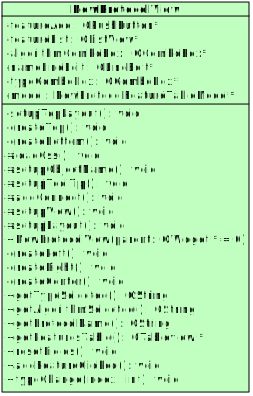
\includegraphics[scale=0.4]{./Images/NewProtocolView}
\caption{\textit{Protocol creation window}}
\label{createprotocolimg}
\end{center}
\end{figure}
\pagebreak
\\The left one contains information about the \protocol{} that is going to be created (Name and Type). The center panel eventually contains a list of feature extractors\g{} that the user has associate to the \protocol{}. Above that list there are the \textit{Add Feature} and the \textit{Remove Selected} buttons. The right one contains the drop-down menu to select the cluster algorithm. In any moment, the user can go back to the main window by selecting the \textit{Back} button.
To create a new Protocol\g{}, follow these instructions:
\begin{itemize}
\item From the \protocol{} creation window, type a unique name in the \textit{Name} field. That name will be the name of the Protocol\g{};
\item Select the type of the Subjects\g{} on which the Protocol\g{} will perform from the \textit{Type} drop-down menu;
\item To add some feature extractors\g{} in the Protocol\g{}, select the \textit{Add Feature} button, and follow these instructions (fig. \ref{featureselector}):
\begin{figure}[!h]
\begin{center}
\includegraphics[scale=0.4]{./Images/FeatureSelector}
\caption{\textit{Feature selector dialog window}}
\label{featureselector}
\end{center}
\end{figure}
\begin{itemize}
\item From the feature selector dialog window, select the feature extractor to include from the drop-down menu. Romeo will show the parameters that have to be setted;
\item Type the necessary parameters for the selected feature or leave the default ones;
\item Select the \textit{Ok} button to confirm the selection.
\end{itemize}
\item To add a cluster algorithm into the Protocol\g{}, select it from the drop-down menu on the right panel of the window and then set the relative parameters;
\item Select the \textit{Save} button to confirm the operation. Romeo will report an error message if the name chosen for the \protocol{} is already present in Romeo or not all the required fields are properly completed.
\end{itemize}

\subsubsection{Manage Protocols}
\label{manageprotocol}
Romeo allows the user to visualize the details of the stored Protocols\g{} and permits their removal. These features are assigned to the Protocols\g{} managing window.\\
From the main window of Romeo, select the \textit{Manage Protocols} button or choose the right one in the toolbar (see \ref{environment}). The Protocols\g{} managing window (fig. \ref{manageprotocolimg}) is composed of two panels. The left one contains the list of Protocols\g{} actually stored in Romeo, while the right one contains the details of the selected \protocol{}. In any moment, the user can go back to the main window by selecting the \textit{Back} button.
\begin{figure}[!h]
\begin{center}
\includegraphics[scale=0.4]{./Images/ViewProtocols}
\caption{\textit{Protocols managing window}}
\label{manageprotocolimg}
\end{center}
\end{figure}

\paragraph{\underline{Visualize Protocol details}:} to visualize the details of a \protocol{}, follow these instructions:
\begin{itemize}
\item From the Protocols\g{} managing window, select the \protocol{} of interest from the list;
\item The details panel will show information about the features extractors\g{} and/or cluster algorithm\g{} associated with the Protocol\g{}.
\end{itemize}

\paragraph{\underline{Modify a Protocol}:} to modify a \protocol{}, follow these instructions:
\begin{itemize}
\item From the Protocols\g{} managing window, select the one that you want to modify;
\item Select the \textit{Edit} button. Romeo will load the fig. \ref{editprotocol} window;
\item From this window it is possible to add or remove some features and/or change the cluster algorithm of the protocol. To perform these actions, follow the instructions of \ref{createprotocol};
\item Confirm the operation by selecting the \textit{Save} button.
\end{itemize}
\begin{figure}[!h]
\begin{center}
\includegraphics[scale=0.4]{./Images/ManageProtocol}
\caption{\textit{Editing a Protocol}}
\label{editprotocol}
\end{center}
\end{figure}

\paragraph{\underline{Delete a Protocol}:} to delete a \protocol{} from Romeo, follow these instructions:
\begin{itemize}
\item From the Protocols\g{} managing window, select the \protocol{} of interest from the list;
\item Select the \textit{Delete} button to confirm the removal.
\end{itemize}
\pagebreak

\subsection{About Datasets}
\label{aboutdatasets}
This section contains the procedures to create and manage the Datasets\g{}.

\subsubsection{Create a Dataset}
\label{createdataset}
The creation of a new Dataset\g{} is assigned to the Dataset\g{} creation window.\\
From the main window of Romeo, select the \textit{New Dataset} button or choose the right one in the toolbar (see \ref{environment}). The Dataset\g{} creation window (fig. \ref{createdatasetimg}), is composed of three panels and a form.\\
The form allow the user to type the name of the Dataset\g{} that will be created. The left panel contains the list of groups of Subjects\g{} actually stored in Romeo, while the center one contains the list of Protocols\g{} (filtered according to the selected group). The right panel contains the details of the selected group of Subject\g{} and Protocol\g{}. In any moment, the user can go back to the main window by selecting the \textit{Back} button.
\begin{figure}[!h]
\begin{center}
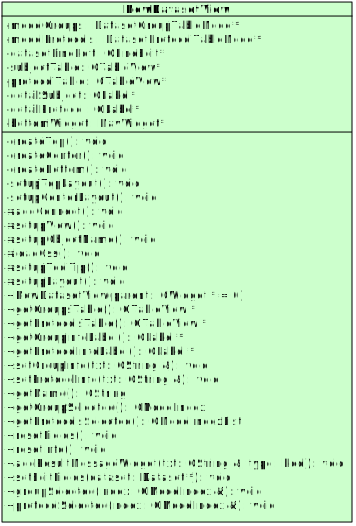
\includegraphics[scale=0.4]{./Images/NewDatasetView}
\caption{\textit{Dataset creation window}}
\label{createdatasetimg}
\end{center}
\end{figure}
To create a new Dataset\g{}, follow these instructions:
\begin{itemize}
\item From the Dataset\g{} creation window, type a unique name in the \textit{Dataset Name} field. That name will be the name of the Dataset\g{};
\item Select the group of Subjects\g{} that have to be associated with the Dataset\g{} from the \textit{Group Of Subjects} panel. Romeo will load the compatible Protocols\g{} in the \textit{Protocols} panel;
\item Select the Protocols\g{} that have to be associated with the Dataset\g{} from the \textit{Protocols} panel;
\item Select the \textit{Save} button to confirm the operation. Romeo will report an error message if the name chosen for the Dataset{} is already present in Romeo.
\end{itemize}

\subsubsection{Manage Datasets}
\label{managedataset}
Romeo allows the user to visualize the details of the stored Datasets\g{} and permits their removal. These features are assigned to the Datasets\g{} managing window.\\
From the main window of Romeo, select the \textit{Manage Datasets} button or choose the right one in the toolbar (see \ref{environment}). The Datasets\g{} managing window (fig. \ref{managedatasetimg}) is composed of two panels. The left one contains the list of Datasets\g{} actually stored in Romeo, while the right one contains the details of the group of Subjects\g{} and Protocols\g{} associated with the selected Dataset\g{}. In any moment, the user can go back to the main window by selecting the \textit{Back} button.
\begin{figure}[!h]
\begin{center}
\includegraphics[scale=0.4]{./Images/ViewDatasets}
\caption{\textit{Datasets managing window}}
\label{managedatasetimg}
\end{center}
\end{figure}

\paragraph{\underline{Visualize Dataset details}:} to visualize the details of a \dataset{}, follow these instructions:
\begin{itemize}
\item From the Datasets\g{} managing window, select the \dataset{} of interest from the list;
\item The details panel will show informations about the groups of Subjects\g{} and the Protocols\g{} associated with the \dataset{}.
\end{itemize}

\paragraph{\underline{Delete a Dataset}:} to delete a \dataset{} from Romeo, follow these instructions:
\begin{itemize}
\item From the Datasets\g{} managing window, select the \dataset{} of interest from the list;
\item Select the \textit{Delete} button to confirm the removal.
\end{itemize}

\pagebreak